\section{Problème 1D}

Dans cette partie, l'objectif est d'exprimer le problème de la propagation acoustique dans une cavité unidimensionnelle
en utilisant le formalisme "éléments finis".

Le schéma du problème est présenté en figure~\ref{fig:FEM:propa_1D}.

\begin{figure}[!ht]
	\centering
	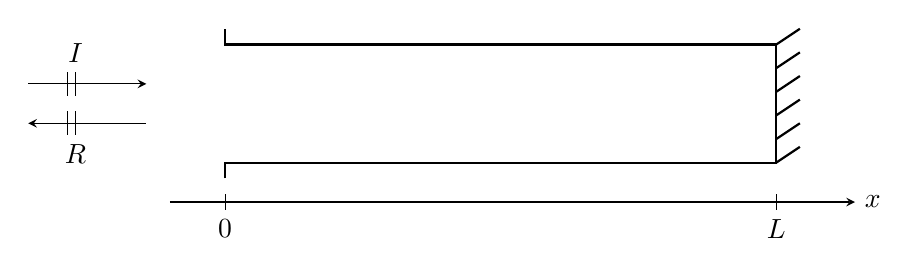
\begin{tikzpicture}[>=stealth]

	% waveguide
	\draw[thick] (0,.3) -- (0,.5) -- (7,.5) -- (7,2) -- (0,2) -- (0,2.2);
	\foreach \i in {0,...,5}{
		\draw[thick] (7,\i*0.3+0.5) -- ++(.3,.2);
	}
	
	% x axis
	\draw[->] (-.7,0) -- (8,0) node[right] {$x$};
	\draw (0,.1) -- ++(0,-.2) node[below] {$0$};
	\draw (7,.1) -- ++(0,-.2) node[below] {$L$};

	% waves
	% R
	\draw[<-] (-2.5,1) -- ++(1.5,0);
	\draw (-2,1.15) -- ++(0,-.3);
	\draw (-1.9,1.15) -- ++(0,-.3) node[below] {$R$};

	% I
	\draw[->] (-2.5,1.5) -- ++(1.5,0);
	\draw (-2,1.65) -- ++(0,-.3);
	\draw (-1.9,1.65) node[above] {$I$} -- ++(0,-.3);

\end{tikzpicture}


	\caption{\label{fig:FEM:propa_1D}Schéma du problème de propagation dans une cavité acoustique 1D de longueur L.}
\end{figure}

\subsection{Position du Problème}

Les conditions aux limites en $x=0$ et $x=L$ imposent :

\begin{equation}
	\left\{\begin{array}{l}
	\left.\nabla p\right|_{x=L} = 0\\
	\left.p\right|_{x=0} = p_i+p_r
	\end{array}\right. \label{FEM1D:BC}
\end{equation}

\subsection{Solution par éléments finis}

En se plaçant dans le formalisme éléments finis, il vient --- d'après~\eqref{FEM1D:final} :

\begin{equation}
	\left[- \uul{K} + k^2\uul{M}\right]\GP = \begin{Bmatrix} \nabla p\bigg|_0\\0\\\vdots\\0\\-\nabla p\bigg|_L\end{Bmatrix}
\end{equation}

En considérant la condition en limite en $x=L$, le second membre est simplifié :

\begin{equation}
\left[- \uul{K} + k^2\uul{M}\right]\GP = \begin{Bmatrix} \nabla p\bigg|_0\\0\\\vdots\\0\end{Bmatrix}
	\label{FEM1D:post_BCL}
\end{equation}

\subsection{Prise en compte de l'excitation}

Le problème est posé de sorte que l'entrée du résonateur est excitée par une onde plane se propageant vers les $x$
croissants et que les interactions à l'interface produisent une onde plane réfléchie se propageant vers les $x$
décroissants. Ainsi, en notant $p_i$ l'onde incidente et $p_r$ l'onde réfléchie :

\begin{equation}
	\left\{
	\begin{array}{l}
		p_i(x) = 1e^{-jk_xx}\\
		p_r(x) = Re^{+jk_xx}
	\end{array}
	\right.\label{FEM1D:expr_ondes}
\end{equation}

La continuité des pressions et des vitesses normales en $x=0$ amène :

\begin{equation*}
	p(0) = e^{-jk_x\times0}+Re^{jk_x\times0} \Leftrightarrow p'(0) = jk(R-1)
\end{equation*}

En remplaçant ce dernier résultat dans~\eqref{FEM1D:final}, il vient :

\begin{equation}
\left[\uul{K} - k^2\uul{M}\right]\GP = \begin{Bmatrix} jk(R-1)  \\0\\\vdots\\0\end{Bmatrix} \label{FEM1D:final}
\end{equation}

Il est alors intéressant de rassembler les inconnues sur la gauche de l'équation en introduisant le vecteur étendu
suivant :

\begin{equation*}
	\ul{X} = [\GP ~|~ R]^T
\end{equation*}

Il est aussi nécéssaire d'étendre la matrice de la partie gauche d'une colonne. Pour maintenir des dimensions cohérentes
dans le système d'équations, il faudra enfin retranscrire la condition de continuité suivante sur la dernière ligne :

\begin{equation*}
	\uul{P}_0 = 1 + R
\end{equation*}

soit :

\begin{equation}
	\underbrace{\left(~
	\begin{array}{cccc|c}
		&&&&-jk\\
		&&&&0\\
		& & \uul{K} - k^2\uul{M} & &\vdots \\
		&&&&0\\\hline
			1 & 0 & \cdots & 0& -1 \\
	\end{array}
	~\right)}_{\uul{A}}
	\underbrace{\left\{~
	\begin{matrix}
		\\
		\\
		\GP\\
		\\\hline
		R
	\end{matrix}
	~\right\}}_{\ul{X}} = 
	\underbrace{\left\{~
	\begin{matrix}
		-jk\\
		0\\
		\vdots\\
		0\\\hline
		1
	\end{matrix}
	~\right\}}_{\ul{b}}
\end{equation}

La résolution se fait alors simplement sur un système de calcul matriciel :

\begin{equation*}
	\ul{X} = \uul{A}^{-1}\ul{b}
\end{equation*}

\subsection{Solution analytique}

Afin d'apprécier la qualité de l'approximation par éléments finis, il est nécessaire de disposer d'une solution
analytique. Le problème est ici posé de sorte que l'impédance en $x=L$ est connue (voir équation~\eqref{FEM1D:ana:ZL}).

\begin{equation}
	Z_L = Z(L) \rightarrow \infty \label{FEM1D:ana:ZL}
\end{equation}

En utilisant la théorie des lignes (et en particulier la formule de l'impédance ramenée), il vient (avec $Z_c =
\rho c$ l'impédance caractéristique):

\begin{eqnarray}
	Z_i = Z(0) 	& = & Z_c \frac{Z_L+jZ_c\tan(kL)}{Z_c + jZ_L\tan(kL)}\notag\\
			    & = & Z_c \frac{Z_L}{Z_L}\frac{1+j\nicefrac{Z_c}{Z_L}\tan(kL)}{\nicefrac{Z_c}{Z_L} + j\tan(kL)}\notag\\
		    Z_i & \overset{Z_L\rightarrow\infty}{\approx} & Z_c\frac{1}{j\tan(kL)}\label{FEM1D:ana:Zi}
\end{eqnarray}

En considérant une onde incidente d'amplitude 1 (en incidence normale) générant, à l'interface, une onde transmise (dans le
résonateur) et une onde réfléchie d'amplitude $R$ (voir le système d'équations~\eqref{FEM1D:expr_ondes}), puis en écrivant les
conditions de continuité, il vient :

\begin{equation*}
	R = \frac{Z_i-Z_c}{Z_i+Z_c}
\end{equation*}

En remplaçant~\eqref{FEM1D:ana:Zi} dans l'équation précédente :

\begin{equation}
	R = \frac{Z_c}{j\tan(k*L)}\label{FEM1D:ana:R}
\end{equation}

\subsection{Convergence}

La suite compare la phase du coefficient de réflexion analytique et celle du coefficient calculé par éléments
finis. L'étude vise à la comparaison des courbes de convergence pour des éléments linéaires et quadratiques.

La fonction d'erreur utilisée mesure l'erreur sur la phase du coefficient de réflexion :

\begin{equation}
	err = \frac{\left|\arg(R) - \arg(\hat{R})\right|^2}{\left|\arg(R)\right|^2}
    \label{FEM1D:errf}
\end{equation}


Les résultats sont présentés en figure~\ref{fig:FEM1D:simuls}.

\begin{figure}[!ht]
	\centering
	\begin{subfigure}{0.48\textwidth}
		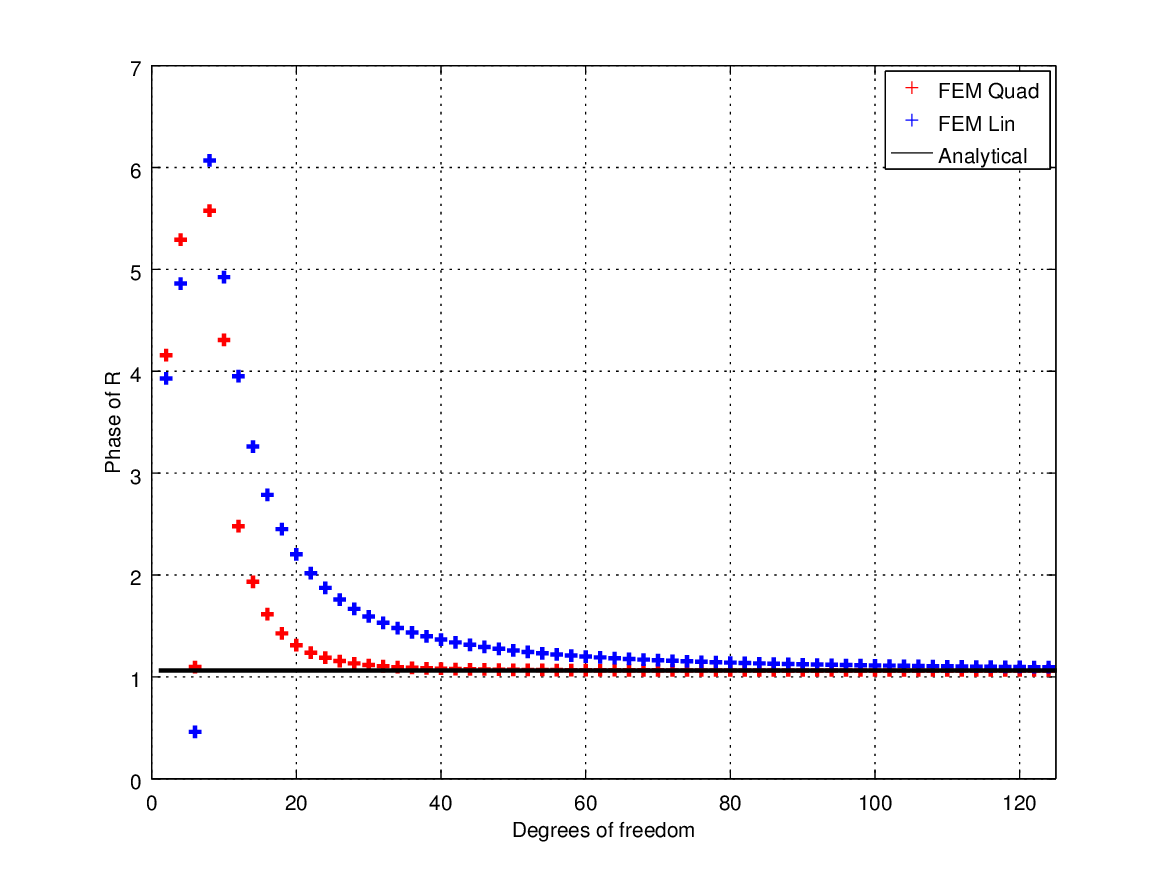
\includegraphics[width=\textwidth]{part1/figs/FEM/simuls_1D/phase.png}
		\caption{\label{fig:FEM1D:simuls:phase}Valeurs de $arg(R)$ en fonction du nombre de degrés de liberté.}
	\end{subfigure}~%
	\begin{subfigure}{0.48\textwidth}
		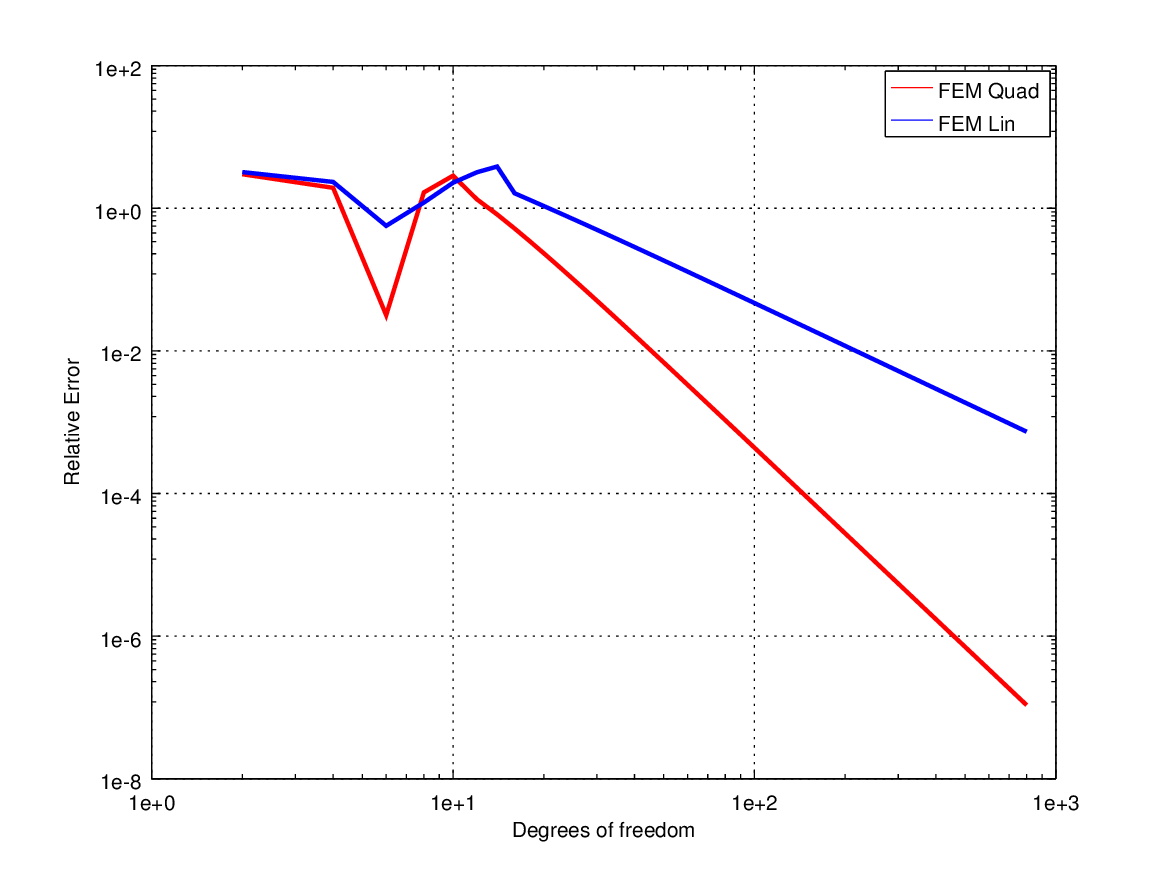
\includegraphics[width=\textwidth]{part1/figs/FEM/simuls_1D/convergence.png}
		\caption{\label{fig:FEM1D:simuls:convergence}Valeurs des fonctions d'erreur en fonction du nombre de degrés de liberté.}
\end{subfigure}
	\caption{\label{fig:FEM1D:simuls}Résultat des simulations. En rouge, les résultats pour des éléments quadratiques en bleu pour des éléments
	linéaires : on remarque une meilleure convergence des premiers (voir figure~\ref{fig:FEM1D:simuls:convergence}). Dans
	les deux cas, la valeur théorique est correctement approchée si l'on augmente le nombre d'éléments.}
\end{figure}

Le passage d'éléments linéaires à des éléments quadratiques augmente d'un ordre la convergence de la méthode, comme le
montre le diagramme de convergence (figure~\ref{fig:FEM1D:simuls:convergence}).

Il faut noter toutefois que dans un cas comme dans l'autre, l'approximation tend vers la solution exacte en augmentant
le nombre d'éléments.

Une autre limite apparaît lorsqu'est considèrée l'influence de la fréquence : en effet, pour une bonne précision de
l'approximation, il est nécessaire de disposer d'au moins 2 éléments par longueur d'onde : les méthodes par éléments
finis sont donc très gourmandes aux hautes fréquences de part la nécessité de disposer d'un maillage toujours plus fin
et donc d'augmenter drastiquement la taille des structures de donnée.

